\documentclass{article}


\usepackage{arxiv}

\usepackage[utf8]{inputenc} % allow utf-8 input
\usepackage[T1]{fontenc}    % use 8-bit T1 fonts
\usepackage{hyperref}       % hyperlinks
\usepackage{url}            % simple URL typesetting
\usepackage{booktabs}       % professional-quality tables
\usepackage{amsfonts}       % blackboard math symbols
\usepackage{nicefrac}       % compact symbols for 1/2, etc.
\usepackage{microtype}      % microtypography
\usepackage{lipsum}
\usepackage{graphicx}
\usepackage{float}
\usepackage{hhline}
\usepackage{gensymb}
\graphicspath{ {./images/} }
\usepackage{caption}
\captionsetup[table]{skip=10pt}

\title{Features of deep learning models in context of semantic segmentation task}


\author{
 Pęczek Paweł \\
  Faculty of Computer Science, Electronics and Telecommunications\\
  AGH University of Science and Technology \\
  Cracow \\
  \texttt{peczek@student.agh.edu.pl} \\
  %% examples of more authors
  \And
 Droński Michał \\
  Faculty of Computer Science, Electronics and Telecommunications\\
  AGH University of Science and Technology \\
  Cracow \\
  \texttt{dronski@student.agh.edu.pl} \\
}

\begin{document}
\maketitle
\begin{abstract}
Deep Learning models have shown their expression power in a wide range of applications including Computer Vision, Natural Language Processing and graph processing. One of the topics that bring attention of researchers is image semantic segmentation which can be seen as a way towards visual scene comprehension. Capability to retrieve context of visual scenes is a key factor contributing success of various practical applications ranging from medical imaging to vehicle autonomy. There are, however, several difficulties that must be overcome to fully solve semantic segmentation challenge in general case, such as modelling diversity of objects scale and their semantic dependencies. In this work we aim to evaluate possibility of training stable semantic segmentation model on relatively small dataset finding a trafe-off between accuracy and computational efficiency. 
\end{abstract}

% keywords can be removed
\keywords{Computer Vision \and Semantic Segmentation \and Deep Learning \and Convolutional Neural Networks}
\raggedbottom
\section{Introduction}
\paragraph{}
Empowered by modern GPU units, Deep Learning (DL) models are able to achieve outstanding performance on wide range of tasks focused on extensive and automatic information retrieval from data in various form. Since AlexNet \cite{alex} was released, the continuous growth of attention on Convolutional Neural Networks (CNNs) development can be observed. CNNs are successfully used to solve many classical Computer Vision (CV) tasks such as image classification. Over years CNNs have proved their tremendous expression power in modelling CV problems ranging from classification to much more sophisticated ones, like semantic segmentation. Despite emergence of other approaches towards modelling visual scenes (e.g. \cite{scae}), conovolutional bias seems still guarantee the best performance in complex CV challenges. In essence, CNN can be seen as an parameterized approximation $f^{*}_{\theta}$ of a function $f: \mathcal{I} \rightarrow \mathcal{T}$ that maps input $i \in \mathcal{I}$ into target $t \in \mathcal{T}$. Domain and range of function $f$ differ w. r. t. specific task. In case of semantic segmentation $\mathcal{I}_{semseg} = \mathbb{R}^{H \times W \times C}$ and $\mathcal{T}_{semseg} = \mathbb{R}^{H \times W \times S}$ ($H, W, C, S$ are images height, width, color chanels and number of semantic classes respectively). Element $t \in \mathcal{T}_{semseg}$ is a pixel-wise map of probability distribution over semantic classes describing which class a pixel belongs to. Parameters $\theta$ are determined while training procedure that is supposed to optimize objective function $J$ formulated in a way specific for a target task. 

\paragraph{}
Research effort on improving current state-of-the-art semantic segmentation methods is important due to possible applications of systems based on models or algorithms that solve the task. Such systems can be utilized to improve autonomous vehicles by ensuring more comprehensive surroundings understanding. What is more, in the field of medical imaging there is a chance to develop systems to assess wide range of scans without human supervision. This application may have tangible effect on the quality of treatment and effectiveness of medical screening. Nevertheless, the general and robust method for solving semantic segmentation challenge is not yet known. The task complexity lays in wide range and high variety of visual scenes that may be segmentation input. Such scenes may contain very different objects both among different possible images and within a particular example. Objects scale variety is also potential challenge. Additionally, a truly robust semantic segmentation solution should also grasp the semantic dependency between objects inside image. For instance high building in urban scene should be recognized as \textit{skyscraper}, whereas large building in industry context probably as \textit{factory}. Unfortunately, CNNs (even particularly deep) cannot solve all mentioned issues without improvements in their architectures or training methods. 

\paragraph{}
In this paper we would like to describe our approach to crealte and train convolutional neural network fo real-time semantic segmentation. Currently, it is not possible to create a complicated model of a convolution network that gives good results while allowing real-time inference with a frequency of several dozen frames per second, so a compromise between the complexity of the model and the inference time is necessary. As part of the task we had at our disposal a very small dataset VISAPP \cite{visapp} containing objects with no backgrounds, belonging to six different classes shown under different angles and a set of backgrounds used for image creation. Limited dataset size forced us to use a large number of synthetic dataset augumentation. We have evaluated and compared two deep learning models: state-of-the-art architecture called  ICNet proposed in \cite{icnet} and one of the first and well-known semantic segmentation network U-Net proposed in\cite{unet}. In addition, we examined how the limited size of a training set affects the quality and stability of model segmentation.

\paragraph{}
The structure of this work is the following. Section \ref{sec:related_work} contain detailed description of state-of-the-art methods for semantic segmentation. In Section \ref{sec:method} we present the research methodology used to obtain results which are outlined in Section \ref{sec:conclusions}. Conclusions, general observations and proposals for further work are presented in Section \ref{sec:conclusions}.  

\section{Related work}
\label{sec:related_work}
\paragraph{}
Presented DL semantic segmentation models usually follow one of two major design approaches. One is to focus on best possible accuracy regardless of computational cost (see Section \ref{sec:gen_methods}) and the other is to optimize models w. r. t. memory footprint and inference speed to enable on-line applications (see Section \ref{sec:rt_methods}).

\subsection{General methods}
\label{sec:gen_methods}
\paragraph{}
One of the first successful approaches towards semantic segmentation was proposed by Shelhamer et al. \cite{fcn}. It uses standard CNN (like LeNet \cite{lenet}, or AlexNet \cite{alex}) as an encoder of image features, but instead of last layers that usually serves as dense classifier, it utilizes convolutional layers, turning the output from fixed-size and non-spatial matrix into classification map. This subtle change allows the FCN to take inputs of any size in contrast to classical CNNs. Shelhamer et al. in \cite{fcn} proposed also the natural way of upsampling features map in a form of backwards strided convolutions so that the model output could be the same size as input. FCN established state-of-the art 62.2\% mIoU accuracy on PASCAL VOC 2012 \cite{pascal_voc}.
\paragraph{}
A natural weakness of previously discussed models is not taking advantage of global context information when solving semantic segmentation task. Zhao et al. proposed PSPNet \cite{psp} that employs pyramid pooling module in order to provide a way to make pixel predictions with regard to scene context. For datasets with a wide range of labels that make the segmentation task significantly complex, global contextual prior is extremally helpful for making accurate predictions. Examples of classes that may be misleading for neural network are described in details in \cite{psp}. Worth noting is the fact that in PSPNet \cite{psp} a CNN output forwarded as an input of pyramid pooling module. Its output after required upsampling is concatenated with original feature map. This kind of modules composition occurs once, after the final convolutional layer of backbone model. A natural extension of this approach should be a desire to inject similar context-aware blocks directly into the encoder network. Regardless of that, the PSPNet \cite{psp} achieved state-of-the art performance in 2017 on CityScapes \cite{cityscapes} (80.2\% mIoU) and PASCAL VOC 2012 \cite{pascal_voc} (85.4\% mIoU). Worth noting also its accuracy (44.94\% mIoU) on significantly hard ADE20K \cite{ade20k} dataset.
\paragraph{}
Another neural network model based shaped in a fully-convolutional fashion was proposed by Ronneberger et al. \cite{unet}. Its architecture is composed of two major parts, named by the authors contracting and expansive paths. The contracting path follows the typical CNN architecture and acts as image features encoder. The second path, on the contrary, serves as decoder and at each step, it consists of upsampling operation followed by convolution. Feature channels number is doubled at each step of contracting path and halved on expansive path. Probability distributions over each pixel of the one before last activation map is produced by convolution with kernel size $1 \times 1$. The whole architecture is U-shaped and additionally employing skip connections between corresponding layers at both paths. Due to the significant difference in the field of applications that U-Net \cite{unet} was designed to, in the original paper there are no evaluation results on datasets like CityScapes \cite{cityscapes} or ADE20K \cite{ade20k}. The value of evaluation metrics mainly discussed in this work is reported only for medical datasets PhC-U373 \cite{phcu373} (92.03\% mIoU) and DIC-HeLa \cite{dichela} (77.56\% mIoU).
\begin{figure}[!htb]
    \centering
  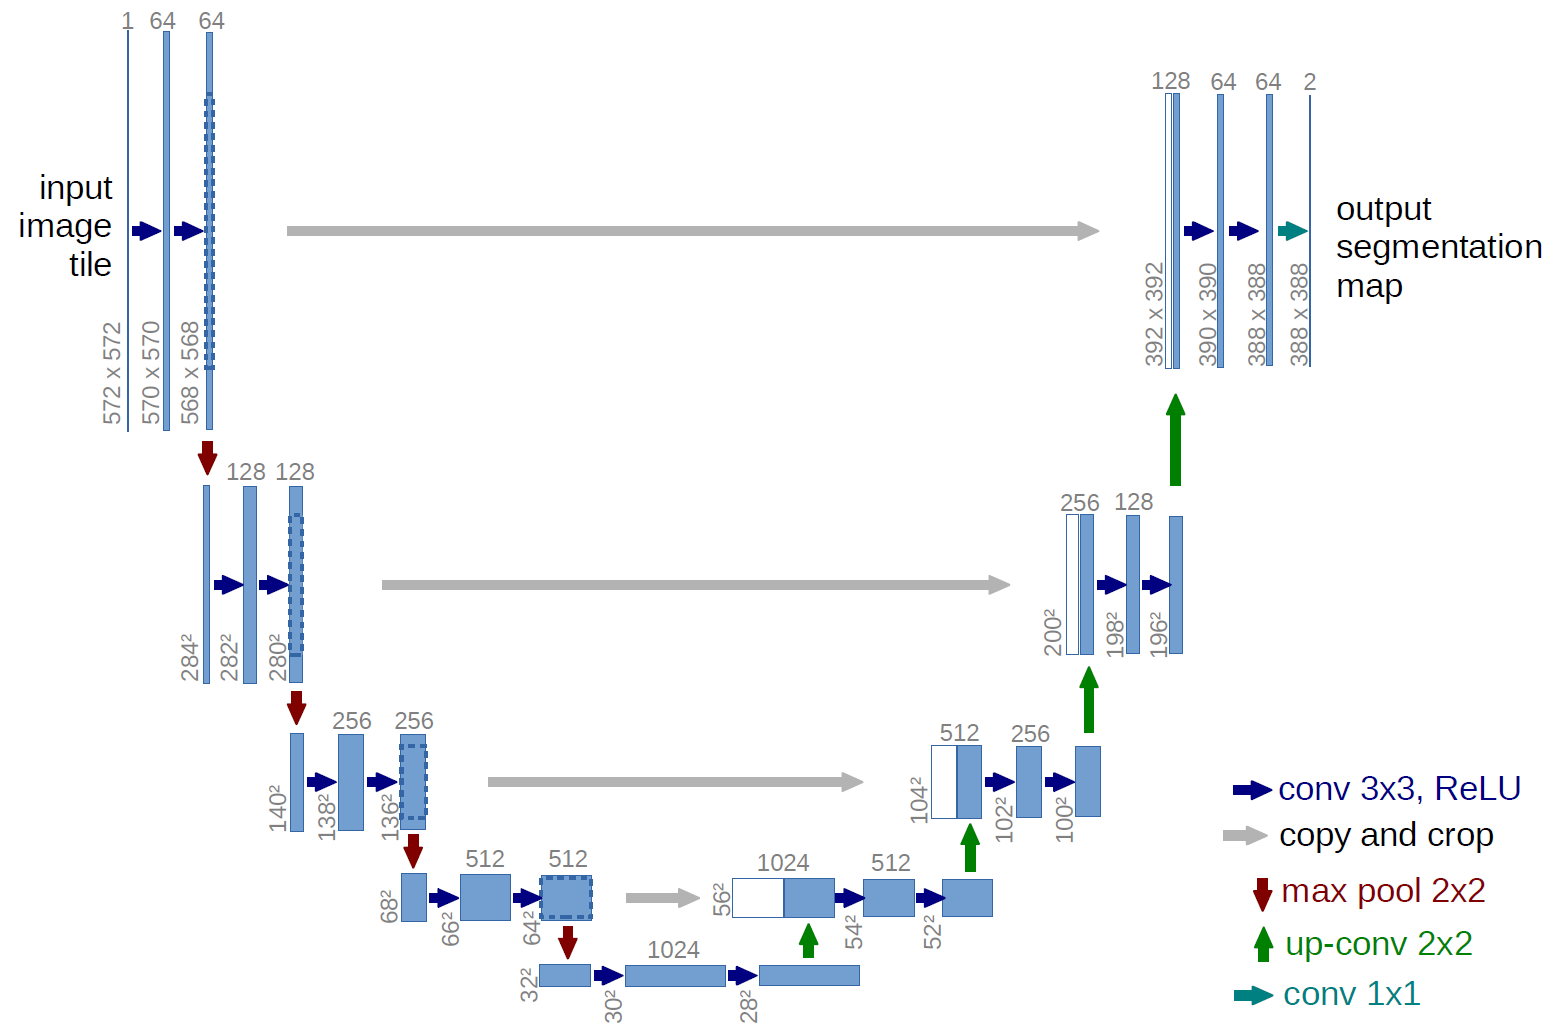
\includegraphics[width=10cm, keepaspectratio]{images/u-net-architecture.png}
  \caption{U-Net~\cite{unet} architecture}
  \label{fig:u-net-architecture}
\end{figure}

\paragraph{}
Slightly different approach was proposed by Guosheng et al. in \cite{refinenet}. Their main assumption was to provide the model multiple paths over which contextual information from different regions of network may be used by the following layers to achieve improvement in segmentation accuracy. In order to reach desired property, the authors proposed the RefineNet architecture. The backbone ResNet \cite{resnet} is divided into 4 blocks with regards to the feature map sizes and serves as an input for RefineNet blocks. Their internal architecture provides a way to fuse feature maps in different resolutions coming from either backbone ResNet or another RefineNet block. RefineNet block as such provides a lot of flexibility in terms of network composition. The architecture described in \cite{refinenet} is therefore only one example of NN possible to be formulated as a part of architectures family that employs RefineNet blocks. Worth noting is the fact that Guosheng et al. in \cite{refinenet} put a lot of effort on ensuring the best possible gradient flow during backpropagation through the RefineNet blocks. Results reported on datasets relevant to this work: Cityscapes \cite{cityscapes} -- 73.6\% mIoU, PASCAL VOC \cite{pascal_voc} -- 83.4\% mIoU, ADE20K \cite{ade20k} -- 40.7\% mIoU.
\paragraph{}
In-depth analysis of ResNet \cite{resnet} architecture was done by Wu et al. in \cite{resnet-revisited}. Based on research conducted, among others, by Szegedy et al. \cite{inception-resnet} and Veit et al. \cite{resnet-enseble}, Wu has shown interesting properties of residual blocks used as basic structure unit of ResNet \cite{resnet}. One of the main field of interest in \cite{resnet-revisited} was to investigate the way that residual networks learn and discover their properties dependent on chosen architecture design. The natural question that arises is about the appropriate trade-off between model width and depth. In the light of findings included in \cite{resnet-revisited} the answer is following. Wider, but quite shallow residual network is able to outperform the deep one, in particular ones that are commonly in use - like ResNet-152 \cite{resnet} or Inception-ResNet \cite{inception-resnet}. Such an architecture could be used both for image classification and (after some changes) semantic segmentation task. The accuracy achieved by the best model proposed in \cite{resnet-revisited} is following. On validation set of CityScapes \cite{cityscapes} -- 77.86\% mIoU. In case of Pascal VOC \cite{pascal_voc} -- 80.84\% mIoU on validation set. On validation set of ADE20K \cite{ade20k} -- 43.73\% mIoU.
\paragraph{}
Wang et al. in \cite{duc} proposed another approach towards architecture of semantic segmentation model. With DUC model they redefined the view on decoder part of a network. The output from standard image feature extractor (like ResNet \cite{resnet}) is prepended by sophisticated functional blocks that are designed to alleviate the detrimental effect of commonly used operations on the model accuracy. Dilated convolutions are widely used as a simple form of enlarging the receptive field of convolutional kernels. Such an approach may enable the possibility to capture characteristics of larger objects without extending the depth of neural network. For tasks like semantic segmentation, this feature may significantly improve the model accuracy. There are, however, downsides of this kind of operations. One of them is called in \cite{duc} "gridding". The phenomenon concerns the basic mechanism that lays behind dilated convolutions. Stacking dilated convolution layers with the fixed dilation rate, it can be observed that information used to compute one particular value of the output feature map is limited only to small fraction of theoretical receptive field. What is more, the alignment of bottom feature maps' regions that influence on it are arranged in a checkerboard fashion. This itself may lead to a mismatch in terms of keeping the local information, as well as to lost of relevant information. As a theoretical solution to this problem Wang et al. proposed a block called \textit{Hybrid Dilated Convolution (HDC)}. It consists of a stack of convolutional layers with different dilation rates chosen carefully such that the convolutional kernels fully cover the region of interest. Authors of \cite{duc} have also raised a problem of feature map upsampling in order to obtain predictions in FCN fashion. As in many concurrent approaches \cite{psp, inception-resnet, icnet} in they discuss the inability of simple bilinear upsampling to adopt to improve the quality of feature maps being processed. However, instead of standard deconvolution operation, Wang et al. proposed \textit{Dense Upsampling Convolution (DUC)}. DUC applies only convolutional operations to get dense prediction map. In order to achieve desired result DUC block outputs the feature map of shape $(H/d) \times (W/d) \times (d^2 + L)$ where $H$ and $W$ are height and width of output prediction respectively, $L$ is the number of classes to predict and $d$ is chosen so that the output map consists of $d^2$ subparts. The output of DUC is reshaped later on to achieve desired size of prediction map. Obtained results clearly show the advantage of DUC both over bilinear upsampling and deconvolutions in terms of ability to restore information from low-resolution feature maps. Results reported on particular datasets are following: CityScapes \cite{cityscapes} -- 80.1\% mIoU, Pascal VOC 2012 \cite{pascal_voc} -- 83.1\% mIoU. 

\subsection{Real-Time methods}
\label{sec:rt_methods}
\paragraph{}
Zhao et al. in \cite{icnet} proposed architecture called ICNet based on the PSPNet \cite{psp} that reaches 30fps on Titan X GPU in high resolution (images from CityScape \cite{cityscapes} sized $1024 \times 2048$). All of this was achieved preserving trade-off between prediction accuracy and inference speed. Considering available time budget the model architecture relies on a cascade of processing pipelines, each operating on input with different resolution and effective feature fusion in \textit{Cascade Fusion Units (CFU)} both with \textit{Cascade Label Guidance (CLG)}. CFU is a sophisticated method for fusion the feature map that comes from different pipelines in such a way that allows to improve coarse, low-resolution prediction and build better, upsampled one. Feature map coming from a lower-resolution stream is upsampled by bilinear interpolation. To improve the quality of upsampling, the dilated convolution is applied directly at the top of it. The result is fused with the second feature map projected by $1 \times 1$ convolution operation. Both feature maps are added up after batch normalization layer being put on top each of them. CLG, on the other hand, is a form of loss function formulation in such manner that encourages intermediate low-resolution feature map to be as close as correspondingly resized ground-truth as possible. Results reported in \cite{icnet} are following: CityScapes \cite{cityscapes} -- 70.6\% mIoU, CamVid \cite{camvid} -- 67.1\% mIoU.
\begin{figure}[!htb]
    \centering
  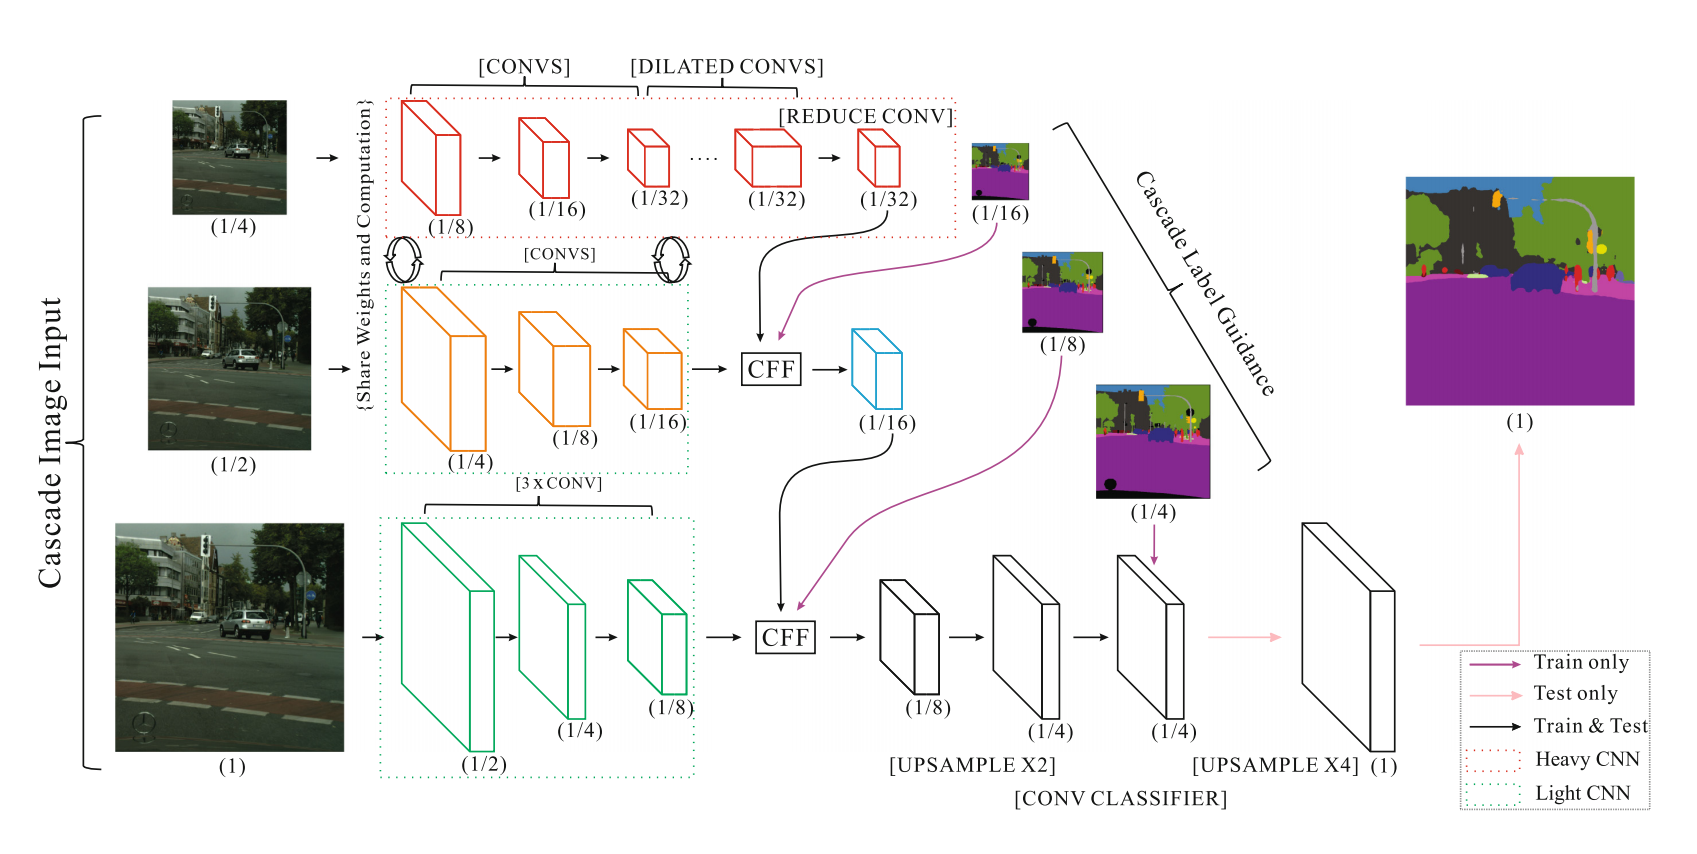
\includegraphics[width=10cm, keepaspectratio]{images/i-cnet-architecture.png}
  \caption{ICNet~\cite{icnet} architecture}
  \label{fig:i-cnet-architecture}
\end{figure}

\paragraph{}
U-shape network architecture used as design pattern when creating various semantic segmentation models (like \cite{icnet}) has few drawbacks. The most important ones are following: a) requirements to operate on high-resolution input feature maps at the initial stages of feed-forward pass and b) weak capacity to recover information from high-resolution branches due to use of low number of convolutional kernels (tight layers). Yu et al. in \cite{bisnet} proposed a different approach based on two major part: Spatial Path (SP) and Context Path (CP). SP handles spatial information preservation whereas CP (Xception-based \cite{xception} architecture) serve as context features extractor. Yu et al. proposed also a new fusion method to improve model performance. In order to ensure large effective receptive field, CP is based on standard, lightweight model (commonly used to solve classification task) followed by Global Average Pooling layer (GAP). What is more, due to refining features of particular CP stages, the authors proposed to use attention-based modules for guiding valuable features learning. Attention-based approach is also used in Feature Fusion Module which merges the results from SP and CP. Thanks to its design, BiSeNet achieves 74.8\% mIoU on CityScapes \cite{cityscapes} (validation set) and 68.7\% mIoU on CamVid \cite{camvid}. Results reported above in terms of CityScapes \cite{cityscapes} evaluation are correct under assumption of full-size (1024x2048) input and real-time regime (NVIDIA Titan XP - 65.5 fps). Without inference time constraints results are better and reaches 80.3\% mIoU on CityScapes \cite{cityscapes} (validation set).

\paragraph{}
Transfer learning is a common practice in wide range of Machine Learning application. Oršić et al. in \cite{swift_net} proposed an architecture utilizing ImageNet pre-trained features to achieve better performance on target task. Pretrained model serves as features encoder, whereas upsampling decoder is jointly trained from scratch on semantic segmentation task. At the end of encoder (in order to increase receptive field under real-time inference regime), simplified version of Spatial Pyramid Pooling block (inspired by one proposed in \cite{psp}) is attached. Decoder is composed of blocks with two inputs - one for previous encoder block output and second for corresponding encoder output (transformed by 1x1 conv). Thanks to ImageNet pretraining, the model achieves 75.5\% mIoU on CityScapes \cite{cityscapes} (validation set) and 39.9 fps inference speed (GTX 1080Ti) on full-size (1024x2048) input. What is more interesting - the same architecture without pretraining achieves  70.4\% mIoU on CityScapes (validation set), which is less than \cite{icnet}. When training without real-time constraint, 76.5\% mIoU on the same dataset was achieved.


\section{Method}
\label{sec:method}
\subsection{Evaluated convolutional neural network models}
\label{sec:evaluated_models}
As part of the task, we evaluated two convolution network architectures: U-Net \cite{unet} and ICnet \cite{icnet}.

It is important to emphasize the significant difference in the number of trainable parameters between ICnet and U-net. Our implementation of ICNet has about 960 000 parameters, which is very small for a convolutional neural network, while U-net has significantly more parameters, as much as about 24 000 000. Comparing the number of parameters, we can see that IOcnet is 25 times smaller than U-net, which suggests that the ICnet will have a much shorter time of inference.


\subsection{Dataset description}
\label{sec:dataset_desc}
The VISAPP~\cite{visapp} data set we use contains six classes presented in \ref{fig:dataset_classes} of objects: \textit{adapter}, \textit{bottle}, \textit{box}, \textit{clamb}, \textit{drill} and \textit{duck}. Each class is divided into subclasses depending on the angle at which the object is presented. Examplary object under different angles is presented in \ref{fig:dataset_examplary_rotations}. All classes are shown at \textit{0\degree}, \textit{30\degree} and \textit{60\degree}, while the adapter and drill additionally at \textit{90\degree}. All elements of the set are raw objects without a background. VISAPP~\cite{visapp} contains an additional folder with backgrounds allowing to generate synthetic images of the same objects on different backgrounds, so there is possibility to  generate far more trainning set elements. Initially, not all classes had annotations about angles, so they were divided into angle subclasses manually.

\begin{center}
\begin{table}[H]
\centering
\tiny \renewcommand{\arraystretch}{2.0}
\begin{tabular}
{ |c|c|c|c|c||c| } \hline Class name & $0\degree$ & $30\degree$ & $60\degree$ & $90\degree$ & $All$  \\ [1.05ex] \hline
$adapter$ &  36 & 36 & 36 & 36 & 144 \\ \hline
$bottle$ &  26 & 27 & 48 & 0 & 101 \\ \hline
$box$ &  12 & 34 & 14 & 0 & 60 \\ \hline
$clamb$ &  12 & 41 & 54 & 0 & 107 \\ \hline
$drill$ &  19 & 36 & 36 & 49 & 140 \\ \hline
$duck$ &  11 & 33 & 50 & 0 & 94 \\ \hline
\end{tabular}
\caption{VISAPP\cite{visapp} dataset distribution}
\label{tab:visapp_class_distribution}
\end{table}
\end{center}


\begin{figure}[!htb]
    \centering
  \includegraphics[width=10cm, keepaspectratio]{images/dataset_examples/classes_cropped.png}
  \caption{Examplary dataset objects withouts backrounds}
  \label{fig:dataset_classes}
\end{figure}

\begin{figure}
    \centering
  \includegraphics[width=10cm, keepaspectratio]{images/dataset_examples/backgrounds_cropped.png}
  \caption{Examplary dataset  backrounds}
  \label{fig:dataset_backgrounds}
\end{figure}

\begin{figure}
    \centering
  \includegraphics[width=10cm, keepaspectratio]{images/dataset_examples/rotations_cropped.png}
  \caption{Examplary dataset object angles}
  \label{fig:dataset_examplary_rotations}
\end{figure}

\subsection{Training strategy}
\label{sec:train_strategy}
We have implemented custom dataset fold generation for training and tests datasets. A single fold consists of a training and test set. The training set was created on the basis of objects present in VISAPP \cite{visapp}, to which random backgrounds were assigned. The images created in this way were subjected to numerous augmentation procedures, among others: \textit{horizontal} \textit{flip}, \textit{vertical flip}, \textit{blur}, \textit{rotation}, \textit{rgb values change}, \textit{grayscale}, \textit{fog}. To check how the model works on real data, images from the test set were not subjected to artificial augmentation.

An important element of the division into training and test set, which should be emphasized, was the arrangement of objects depending on their angle. Table~\ref{tab:rotation_splits} shows how particular train test rotation splits were chosen.
We knew that by dividing the dataset in the above way, we would disrupt train-test ditribution, assuming theoretically recommended random division of the base dataset into train and test sets. We decided to do this to check how roboust the models evaluated by us are. The introduction of such a disturbance in the distribution between the train and test sets also allowed us to check how models trained on a small amount of data generalize to the change in perspective under which the analyzed object is shown.

We evaluated both neural networks described in \ref{sec:evaluated_models} on such prepared data sets. Both models have previously been adapted to the VISAPP \cite{visapp} dataset. ICnet and Unet were trained and validated on the same data sets within the same fold. The training process consisted of 32 epochs on the learning set. K-Fold validation was used for results corectness check.

\begin{center}
\begin{table}[H]
\centering
\tiny \renewcommand{\arraystretch}{1.5}
\begin{tabular}
{ |c||c|c||c|c||c|c| } \hline Class name & $Train^{rot1}$ & $Test^{rot1}$ & $Train^{rot2}$ & $Test^{rot2}$ & $Train^{rot3}$ & $Test^{rot3}$\\ [1.05ex] \hline
$adapter$ &  0, 30, 90 & 60 & 0, 60, 90 & 30 & 30, 60, 90 & 0 \\ \hline
$bottle$ &  0, 60 & 30 & 0, 30 & 60 & 30, 60 & 0 \\ \hline
$box$ &  0, 60 & 30 & 0, 30 & 60 & 30, 60 & 0 \\ \hline
$clamb$ &  0, 60 & 30 & 0, 30 & 60 & 30, 60 & 0 \\ \hline
$drill$ &  0, 30, 90 & 60 & 0, 60, 90 & 30 & 30, 60, 90 & 0 \\ \hline
$duck$ &  0, 60 & 30 & 0, 30 & 60 & 30, 60 & 0 \\ \hline
\end{tabular}
\caption{VISAPP~\cite{visapp} rotation train-test splits}
\label{tab:rotation_splits}
\end{table}
\end{center}

\subsection{Evaluation strategy}
\label{sec:eval_strategy}
\paragraph{}
In binary segmentation setup, Dice coefficient serves as segmentation efficiency metrics in a very natural manner. Assuming objects of interests presence on segmented scene, Dice can be used as evaluation metrics without any adjustments. There are, however, several difficulties that must be overcome when it comes to multi-class generalization of Dice coefficient in context of semantic segmentation model evaluation. One of such issue can be lack of presence of a particular class representative on a particular image under evaluation. Model that predicts perfectly fine result yield \textit{NaN} value of Dice score. The issue can be easily solved by setting Dice score as 1.0 in such cases. On the other hand, if a model output contains negligibly small amount of positive values (taking into account the same setup), the Dice score is 0.0 which seems not to be a fair outcome. Allowing small \textit{noise level $\epsilon$} representing the fraction of output to be \textit{$FP$} for a particular class if this class does not occur in \textit{ground-truth} can efficiently solve this issue. Yet another issue that may occur is the following. Assuming that a particular image does only contain one class instance(s) and the model is evaluated w. r. t. $N$ segmentation classes, in case that a model performs badly on this image and produces only $FN$ values, then the Dice score value for this class is 0.0. The level on how meaningful this value is in the overall score (among all classes) depends on the evaluation strategy. If the chosen approach is to average the score among all classes, then with growth of $N$, the influence of value 0.0 decreases (to the level of being almost impossible to notice). To alleviate such cases, final score averaging should be done only w. r. t. classes actually present in the picture and those one that were predicted by a model (possibly with small noise-level acceptance strategy described above).
\paragraph{}
In the light of potential issues discussion conducted above we would like to outline the evaluation strategy applied on results of our experiments. First of all, we decided to train two models - ICNet \cite{icnet} and U-Net \cite{unet} with and without naive and unconstrained Dice loss coefficient. The loss term always present is cross-entropy. Putting explicit and unconstrained Dice coefficient was intended to validate the differences in training outcomes. Final scores presented in Section \ref{sec:results} are calculated both per-class and w. r. t. all classes in data set (with additional \textit{background} class). We provided two set of results - one averaged on \textit{pixel-wise} level and \textit{example-wise} one. \textit{Example-wise} averaging means using binary weights $w_b^{i, c}$ for all examples $i$ and classes $c$ when calculating Dice score. Value $1$ was assigned to an example $i$ in context of a particular class $c$ if a class was present either in \textit{ground-truth} or \textit{prediction} (in case of prediction - above noise level $\epsilon$). \textit{Pixel-wise} averaging means using as weights $w_p^{i, c}$ values calculated as $TP + FP + FN$ (the only ones that Dice takies into account) for a particular example $i$ and class $c$ (noise tolerance was also applied on prediction). Noise tolerance was 24 pixels per image (as $\epsilon = 0.0015$ and images size was $128 \times 128$). Background class was treated as equally important as other ones.
\paragraph{}
As a result, Dice score for a particular class $c$ was calculated as:
\begin{itemize}
    \item $D^{pw}_{c} = \frac{\sum_i w_p^{i, c}d_i}{\sum_i w_p^{i, c}}$ in case of \textit{pixel-wise} averaging w. r. t. a particular class $c$,
    \item $D^{ew}_{c} = \frac{\sum_i w_b^{i, c}d_i}{\sum_i w_b^{i, c}}$ in case of \textit{example-wise} averaging w. r. t. a particular class $c$,
    \item $D^{pw} = \frac{\sum_{c}\sum_i w_p^{i, c}d_i}{\sum_{c}\sum_i w_p^{i, c}}$ in case of \textit{pixel-wise} averaging w. r. t. all classes,
    \item $D^{ew} = \frac{\sum_{c}\sum_i w_b^{i, c}d_i}{\sum_{c}\sum_i w_b^{i, c}}$ in case of \textit{pixel-wise} averaging w. r. t. all classes.
\end{itemize}
where $d_i$ is Dice score constrained w. r. t. noise tolerance $\epsilon$. 

\paragraph{}
For clarity of results presentation we utilized the following abbreviations for class names: \textit{background - bg}, \textit{box - bx}, \textit{clamp - cl}, \textit{drill - dr}, \textit{duck - du}, \textit{adapter - ad} and \textit{bottle - bo}.

\section{Results}
\label{sec:results}
\paragraph{}
Experiments results determined in regime described in Section \ref{sec:eval_strategy} are presented in Tables \ref{tab:icnet_ce_results} -- \ref{tab:unet_ce_dice_results}. In contrast to majority model performance reports, highlighted values are the worst among detected ones. Majority of worst results (regarding Tables \ref{tab:icnet_ce_results} -- \ref{tab:unet_ce_dice_results} columns) in a number of 88\% are connected with \textit{camera rotation-based} splits of data set. Such phenomenon was supposed to occur due to mismatch in train-test data distribution, but its scale can be seen as a measurement of how weak the models are when it comes to data generalization. The \textit{camera rotation-based} splits were chosen in such a way to test models on unseen angles that are only slightly different from ones that were seen by model while training.  Interestingly, the lowest score values (in terms of absolute magnitude) can be observed in case of $rot_1$. This particular split was created in a way that training set contains extreme angles values and test set - the ones from the middle of available range, so the results are rather  counter-intuitive. There are cases where absolute difference in score magnitude between \textit{random-} and \textit{rotation-based} splits are above $0.35$.

\paragraph{}
In this work we do not aim to compare ICNet \cite{icnet} and U-Net \cite{unet} architectures head-to-head for several different reasons. First of all, according to results reported in Tables \ref{tab:icnet_ce_results} -- \ref{tab:unet_ce_dice_results}, VISAPP \cite{visapp} data set seems not to be sufficiently complex to draw meaningful conclusions regarding particular model features (such conclusions could be drawn rather from meta-analysis than a single experiment). Second of all, those two models differ by large in terms of parameters number. Our version of ICNet \cite{icnet} has less than 1M parameters, whereas our version of U-Net \cite{unet} - more than 20M. This factor contributes significantly not only in computational cost of model inference, but also in model stability. Despite the fact that particularly weak predictions can be observed in case of both models, model with less number of parameters tends to produce less stable output (part of strange model predictions can be influenced by augmentation, but augmentation was needed due to small data set size).

\begin{figure}
    \centering
  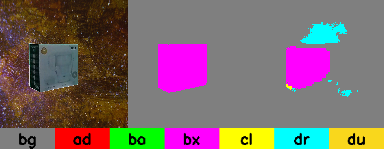
\includegraphics[width=10cm, keepaspectratio]{images/icnet_bad.png}
  \caption{Example of bad prediction from ICNet \cite{icnet} model. In relatively easy case, model predicted three different classes to be present. Picture alignment is the following: from left to right - original example, ground truth and prediction.}
  \label{fig:icnet_bad}
\end{figure}

\paragraph{}
Worth mentioning is the fact that particular classes can be easier to learn that other ones. An example of such class can be \textit{duck}. Objects that belong to this class have characteristic color and shape that is compact and relatively easily to describe. There are, however, classes that are quite challenging for both models, like \textit{box}, \textit{clamp}. The reason those classes are problematic is quite different. In case of \textit{box} class, objects are relatively simple in terms of shape (the shape is even less sophisticated than in terms of \textit{duck}). The reason why models cannot predict segmentation map for \textit{box} instances is probably the objects color in correspondence to backgrounds. The assumption is originated in a fact that even for \textit{human expert} it is harder to visually separate object from background if the object is similar in terms of color to the background. Regardless of the true reason for this phenomenon, its presence indicates how data set complexity influence results (similar conclusions can be drawn from evaluating results achieved by \textit{state-of-the-art} models on CityScapes \cite{cityscapes} in contrast to ones reported foe ADE20K \cite{ade20k} - see Section \ref{sec:related_work}). On the other hand, \textit{clamp} class contain objects which are the most complex in terms of shape among all classes in VISAPP \cite{visapp} data set, what seems to explain the magnitude of difficulties in training phase for a model to learn how to produce stable predictions in case of this particular class. Additionally, in some cases (like U-Net \cite{unet} trained only with CE loss - see Table \ref{tab:unet_ce_results}) \textit{clamp} class tends to be predicted instead of proper classes that should be assigned by a model. Cases like that are source of low $D^{ew}_{c}$ scores. Issues discussed in this paragraph are illustrated on Figure \ref{fig:problematic_cases}.

\begin{figure}
    \centering
  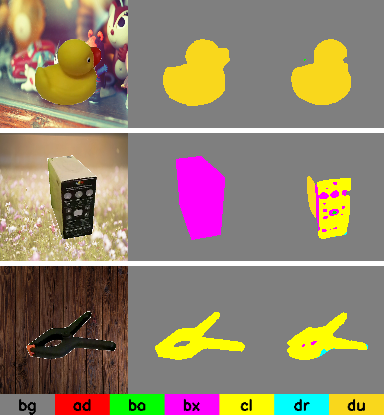
\includegraphics[width=10cm, keepaspectratio]{images/problematic_cases.png}
  \caption{Predictions from U-Net \cite{unet} trained only with CE loss term (see results in Table \ref{tab:unet_ce_results}). For each example (from top to bottom), original image, ground truth and model prediction (from left to right) are presented. First case shows relatively good model prediction on not challenging class (beak of a duck is not predicted correctly, probably due to similarity to background region) even if background contain other objects. Second case shows totally mismatched prediction for a problematic class. It also illustrates the situation when other classes are predicted incorrectly which lowers $D^{ew}_{c}$ scores significantly. Third case illustrates the model issues with predicting proper segmentation map for some areas of \textit{clamp} instance, where object shape is complex and background have similar color to foreground.}
  \label{fig:problematic_cases}
\end{figure}

\begin{center} 
\begin{table}[H]
\tiny \renewcommand{\arraystretch}{1.5} \begin{tabular}{ |c|c|c|c|c|c|c|c|c||c|c|c|c|c|c|c|c| } \hline Split name & $D^{pw}_{bg}$ & $D^{pw}_{bx}$ & $D^{pw}_{cl}$ & $D^{pw}_{dr}$ & $D^{pw}_{du}$ & $D^{pw}_{ad}$ & $D^{pw}_{bo}$ & $D^{pw}$ &  $D^{ew}_{bg}$ & $D^{ew}_{bx}$ & $D^{ew}_{cl}$ & $D^{ew}_{dr}$ & $D^{ew}_{du}$ & $D^{ew}_{ad}$ & $D^{ew}_{bo}$ & $D^{ew}$ \\ [1.05ex] \hline 
$random_0$ &  0.99 & 0.84 & 0.86 & 0.87 & 0.96 & 0.82 & 0.88 & 0.97 &  0.99 & 0.49 & 0.54 & 0.79 & 0.77 & 0.81 & 0.88 & 0.83 \\ \hline 
$random_1$ &  0.99 & 0.8 & \textbf{0.73} & 0.83 & 0.96 & 0.92 & 0.9 & 0.97 &  0.99 & 0.59 & 0.48 & 0.49 & 0.8 & 0.71 & 0.69 & 0.76 \\ \hline 
$random_2$ &  0.99 & 0.83 & 0.82 & 0.83 & 0.97 & 0.92 & 0.85 & 0.97 &  0.99 & 0.4 & 0.48 & 0.56 & 0.97 & 0.72 & 0.85 & 0.77 \\ \hline 
$random_3$ &  0.99 & 0.84 & 0.86 & 0.88 & 0.97 & 0.77 & 0.87 & 0.97 &  0.99 & 0.4 & 0.53 & 0.69 & 0.97 & 0.76 & 0.83 & 0.81 \\ \hline 
$random_4$ &  0.99 & 0.79 & 0.78 & 0.86 & 0.97 & 0.91 & 0.84 & 0.97 &  0.99 & 0.65 & \textbf{0.36} & 0.83 & 0.88 & 0.78 & 0.4 & 0.74 \\ \hline 
$random_5$ &  0.99 & 0.86 & 0.82 & 0.81 & 0.95 & 0.88 & 0.88 & 0.97 &  0.99 & 0.48 & 0.52 & 0.62 & \textbf{0.54} & 0.85 & 0.57 & 0.76 \\ \hline 
$random_6$ &  0.99 & 0.85 & 0.77 & 0.79 & 0.95 & 0.9 & 0.87 & 0.97 &  0.99 & 0.38 & 0.37 & 0.65 & 0.96 & 0.87 & 0.8 & 0.77 \\ \hline 
$random_7$ &  0.99 & 0.7 & 0.75 & 0.83 & 0.96 & 0.93 & 0.9 & 0.97 &  0.99 & 0.57 & 0.37 & 0.56 & 0.88 & 0.93 & 0.68 & 0.77 \\ \hhline{|=|=|=|=|=|=|=|=|=|=|=|=|=|=|=|=|=|} 
$rot_0$ &  \textbf{0.98} & 0.46 & 0.74 & 0.74 & \textbf{0.89} & 0.84 & 0.85 & \textbf{0.95} &  \textbf{0.98} & 0.39 & 0.37 & 0.59 & 0.62 & 0.84 & 0.44 & \textbf{0.69} \\ \hline 
$rot_1$ &  \textbf{0.98} & \textbf{0.42} & 0.78 & 0.72 & 0.96 & 0.82 & 0.79 & 0.96 &  \textbf{0.98} & \textbf{0.13} & 0.6 & 0.51 & 0.88 & \textbf{0.53} & 0.62 & 0.72 \\ \hline 
$rot_2$ &  \textbf{0.98} & 0.9 & 0.82 & \textbf{0.67} & 0.94 & \textbf{0.59} & \textbf{0.72} & \textbf{0.95} &  \textbf{0.98} & 0.9 & 0.65 & \textbf{0.43} & 0.58 & 0.58 & \textbf{0.36} & \textbf{0.69} \\ \hline 
\end{tabular} 
\caption{Results of adjusted ICNet \cite{icnet} model (CE loss) evaluation w. r. t. evaluation strategy described in Section \ref{sec:eval_strategy}. Table rows are indexed by \textit{split name}, where $random_i$ refers to randomly generated split of data set (with randomly adjusted backgrounds) and $rot_i$ refers to data set split prepared w. r. t. angle that a particular image was taken regarding to object. Values marked as \textbf{bold} in particular columns highlight the weakest score in both for \textit{pixel-wise} and \textit{example-wise} score averaging.}
\label{tab:icnet_ce_results}
\end{table}
\end{center}


\begin{center}
\begin{table}[H]
\tiny \renewcommand{\arraystretch}{1.5} \begin{tabular}{ |c|c|c|c|c|c|c|c|c||c|c|c|c|c|c|c|c| } \hline Split name & $D^{pw}_{bg}$ & $D^{pw}_{bx}$ & $D^{pw}_{cl}$ & $D^{pw}_{dr}$ & $D^{pw}_{du}$ & $D^{pw}_{ad}$ & $D^{pw}_{bo}$ & $D^{pw}$ &  $D^{ew}_{bg}$ & $D^{ew}_{bx}$ & $D^{ew}_{cl}$ & $D^{ew}_{dr}$ & $D^{ew}_{du}$ & $D^{ew}_{ad}$ & $D^{ew}_{bo}$ & $D^{ew}$ \\ [1.05ex] \hline 
$random_0$ &  0.99 & 0.87 & 0.75 & 0.82 & 0.95 & 0.9 & 0.87 & 0.97 &  0.99 & 0.8 & 0.32 & 0.74 & 0.74 & 0.82 & 0.59 & 0.76 \\ \hline 
$random_1$ &  0.99 & 0.76 & 0.8 & 0.84 & 0.97 & 0.88 & 0.78 & 0.97 &  0.99 & 0.41 & 0.46 & 0.69 & 0.97 & 0.71 & 0.4 & 0.74 \\ \hline 
$random_2$ &  0.99 & 0.89 & 0.85 & 0.85 & 0.98 & 0.89 & 0.9 & 0.98 &  0.99 & 0.64 & 0.48 & 0.7 & 0.88 & 0.86 & 0.76 & 0.83 \\ \hline 
$random_3$ &  0.99 & 0.85 & 0.85 & 0.86 & 0.97 & 0.8 & 0.89 & 0.98 &  0.99 & 0.84 & 0.48 & 0.66 & 0.77 & 0.64 & 0.7 & 0.79 \\ \hline 
$random_4$ &  0.99 & 0.9 & 0.88 & 0.87 & 0.97 & 0.89 & 0.92 & 0.98 &  0.99 & 0.66 & 0.62 & 0.53 & 0.97 & 0.89 & 0.84 & 0.83 \\ \hline 
$random_5$ &  0.99 & 0.91 & 0.9 & 0.83 & 0.97 & 0.81 & 0.8 & 0.98 &  0.99 & 0.63 & 0.79 & 0.58 & 0.97 & 0.8 & \textbf{0.39} & 0.78 \\ \hline 
$random_6$ &  0.99 & 0.87 & 0.78 & 0.81 & 0.97 & 0.9 & 0.84 & 0.97 &  0.99 & 0.54 & 0.45 & 0.59 & 0.97 & 0.82 & 0.44 & 0.76 \\ \hline 
$random_7$ &  0.99 & 0.67 & 0.68 & 0.8 & 0.96 & 0.94 & 0.87 & 0.97 &  0.99 & 0.38 & 0.39 & 0.63 & 0.92 & 0.88 & 0.42 & 0.74 \\ \hhline{|=|=|=|=|=|=|=|=|=|=|=|=|=|=|=|=|=|}  
$rot_0$ &  \textbf{0.98} & 0.43 & 0.75 & 0.74 & 0.97 & \textbf{0.78} & 0.83 & \textbf{0.95} &  \textbf{0.98} & 0.4 & 0.39 & 0.52 & 0.95 & 0.78 & 0.44 & 0.71 \\ \hline 
$rot_1$ &  \textbf{0.98} & \textbf{0.2} & 0.72 & 0.65 & 0.95 & 0.87 & \textbf{0.77} & \textbf{0.95} & \textbf{0.98} & \textbf{0.09} & 0.46 & \textbf{0.4} & 0.77 & \textbf{0.58} & 0.71 & 0.7 \\ \hline 
$rot_2$ &  \textbf{0.98} & 0.8 & \textbf{0.66} & \textbf{0.63} & \textbf{0.82} & 0.87 & 0.85 & 0.96 &  \textbf{0.98} & 0.74 & \textbf{0.27} & 0.44 & \textbf{0.5} & 0.79 & 0.5 & \textbf{0.69} \\ \hline 
\end{tabular}
\caption{Results of adjusted ICNet \cite{icnet} model (CE + Dice loss) evaluation w. r. t. evaluation strategy described in Section \ref{sec:eval_strategy}. Table rows are indexed by \textit{split name}, where $random_i$ refers to randomly generated split of data set (with randomly adjusted backgrounds) and $rot_i$ refers to data set split prepared w. r. t. angle that a particular image was taken regarding to object. Values marked as \textbf{bold} in particular columns highlight the weakest score in both for \textit{pixel-wise} and \textit{example-wise} score averaging.}
\label{tab:icnet_ce_dice_results}
\end{table}
\end{center}


\begin{center}
\begin{table}[H]
\tiny \renewcommand{\arraystretch}{1.5} \begin{tabular}{ |c|c|c|c|c|c|c|c|c||c|c|c|c|c|c|c|c| } \hline Split name & $D^{pw}_{bg}$ & $D^{pw}_{bx}$ & $D^{pw}_{cl}$ & $D^{pw}_{dr}$ & $D^{pw}_{du}$ & $D^{pw}_{ad}$ & $D^{pw}_{bo}$ & $D^{pw}$ &  $D^{ew}_{bg}$ & $D^{ew}_{bx}$ & $D^{ew}_{cl}$ & $D^{ew}_{dr}$ & $D^{ew}_{du}$ & $D^{ew}_{ad}$ & $D^{ew}_{bo}$ & $D^{ew}$ \\ [1.05ex] \hline 
$random_0$ &  0.99 & 0.59 & 0.65 & 0.68 & 0.95 & 0.89 & 0.82 & 0.96 &  0.99 & 0.5 & 0.36 & 0.36 & 0.91 & 0.75 & 0.44 & 0.67 \\ \hline 
$random_1$ &  0.99 & 0.68 & 0.74 & 0.71 & 0.95 & 0.8 & 0.79 & 0.96 &  0.99 & 0.5 & 0.38 & 0.4 & 0.54 & 0.54 & 0.64 & 0.66 \\ \hline 
$random_2$ &  0.98 & 0.48 & 0.68 & 0.66 & 0.96 & 0.88 & 0.74 & 0.95 &  0.98 & 0.13 & 0.32 & 0.34 & 0.96 & 0.59 & 0.31 & 0.54 \\ \hline 
$random_3$ &  0.98 & 0.6 & 0.65 & 0.72 & 0.92 & 0.82 & 0.75 & 0.96 &  0.98 & 0.23 & 0.29 & 0.5 & 0.44 & 0.48 & 0.38 & 0.58 \\ \hline 
$random_4$ &  0.99 & 0.79 & 0.78 & 0.77 & 0.95 & 0.91 & 0.8 & 0.97 &  0.99 & 0.33 & 0.32 & 0.51 & 0.76 & 0.67 & 0.32 & 0.63 \\ \hline 
$random_5$ &  0.99 & 0.72 & 0.74 & 0.72 & 0.95 & 0.93 & 0.84 & 0.97 &  0.99 & 0.47 & 0.31 & 0.42 & 0.95 & 0.78 & 0.45 & 0.68 \\ \hline 
$random_6$ &  0.99 & 0.55 & 0.6 & 0.68 & 0.95 & 0.9 & 0.82 & 0.96 &  0.99 & 0.54 & 0.29 & 0.53 & 0.82 & 0.66 & 0.55 & 0.69 \\ \hline 
$random_7$ &  0.98 & 0.55 & 0.7 & 0.63 & 0.87 & 0.84 & 0.71 & 0.95 &  0.98 & 0.32 & 0.34 & 0.38 & 0.45 & 0.51 & 0.3 & 0.58 \\ \hhline{|=|=|=|=|=|=|=|=|=|=|=|=|=|=|=|=|=|}   
$rot_0$ &  \textbf{0.97} & 0.35 & 0.56 & \textbf{0.5} & 0.93 & 0.88 & 0.75 & \textbf{0.93} & \textbf{0.97} & 0.33 & 0.31 & \textbf{0.22} & 0.83 & 0.73 & 0.47 & 0.62 \\ \hline 
$rot_1$ &  0.98 & \textbf{0.12} & 0.66 & 0.63 & 0.93 & \textbf{0.68} & \textbf{0.68} & 0.94 &  0.98 & \textbf{0.07} & 0.49 & 0.28 & 0.82 & \textbf{0.38} & 0.55 & 0.63 \\ \hline 
$rot_2$ &  0.98 & 0.52 & \textbf{0.49} & 0.64 & \textbf{0.74} & 0.81 & 0.7 & 0.94 &  0.98 & 0.18 & \textbf{0.18} & 0.33 & \textbf{0.38} & 0.52 & \textbf{0.27} & \textbf{0.49} \\ \hline 
\end{tabular} 
\caption{Results of adjusted U-Net \cite{unet} model (CE loss) evaluation w. r. t. evaluation strategy described in Section \ref{sec:eval_strategy}. Table rows are indexed by \textit{split name}, where $random_i$ refers to randomly generated split of data set (with randomly adjusted backgrounds) and $rot_i$ refers to data set split prepared w. r. t. angle that a particular image was taken regarding to object. Values marked as \textbf{bold} in particular columns highlight the weakest score in both for \textit{pixel-wise} and \textit{example-wise} score averaging.}
\label{tab:unet_ce_results}
\end{table}
\end{center}

\begin{center}
\begin{table}[H]
\tiny \renewcommand{\arraystretch}{1.5} \begin{tabular}{ |c|c|c|c|c|c|c|c|c||c|c|c|c|c|c|c|c| } \hline Split name & $D^{pw}_{bg}$ & $D^{pw}_{bx}$ & $D^{pw}_{cl}$ & $D^{pw}_{dr}$ & $D^{pw}_{du}$ & $D^{pw}_{ad}$ & $D^{pw}_{bo}$ & $D^{pw}$ &  $D^{ew}_{bg}$ & $D^{ew}_{bx}$ & $D^{ew}_{cl}$ & $D^{ew}_{dr}$ & $D^{ew}_{du}$ & $D^{ew}_{ad}$ & $D^{ew}_{bo}$ & $D^{ew}$ \\ [1.05ex] \hline 
$random_0$ &  0.99 & 0.72 & 0.64 & 0.76 & 0.96 & 0.85 & 0.87 & 0.97 &  0.99 & 0.48 & 0.38 & 0.42 & 0.96 & 0.85 & 0.61 & 0.73 \\ \hline 
$random_1$ &  0.99 & 0.79 & \textbf{0.58} & 0.68 & 0.96 & 0.88 & 0.88 & 0.97 &  0.99 & 0.32 & 0.37 & 0.47 & 0.71 & 0.76 & 0.67 & 0.71 \\ \hline 
$random_2$ &  0.99 & 0.82 & 0.71 & 0.79 & 0.95 & 0.86 & 0.89 & 0.97 &  0.99 & 0.35 & 0.37 & 0.46 & 0.61 & 0.73 & 0.57 & 0.68 \\ \hline 
$random_3$ &  0.99 & 0.7 & 0.71 & 0.85 & 0.96 & 0.86 & 0.82 & 0.97 &  0.99 & 0.17 & 0.24 & 0.65 & 0.92 & 0.51 & 0.46 & 0.58 \\ \hline 
$random_4$ &  0.99 & 0.75 & 0.59 & 0.62 & 0.93 & 0.9 & 0.86 & 0.96 &  0.99 & 0.55 & 0.38 & 0.41 & 0.44 & 0.66 & 0.48 & 0.66 \\ \hline 
$random_5$ &  0.99 & 0.69 & 0.64 & 0.8 & 0.95 & \textbf{0.73} & 0.72 & 0.96 &  0.99 & 0.23 & \textbf{0.28} & 0.58 & 0.9 & 0.69 & \textbf{0.32} & 0.62 \\ \hline 
$random_6$ &  0.99 & 0.49 & 0.59 & 0.77 & 0.95 & 0.81 & 0.88 & 0.96 &  0.99 & 0.2 & 0.31 & 0.48 & 0.82 & \textbf{0.46} & 0.74 & 0.65 \\ \hline 
$random_7$ &  0.99 & 0.46 & 0.65 & 0.75 & 0.96 & 0.89 & 0.8 & 0.96 &  0.99 & 0.15 & \textbf{0.28} & 0.5 & 0.76 & 0.64 & 0.38 & \textbf{0.61} \\ \hhline{|=|=|=|=|=|=|=|=|=|=|=|=|=|=|=|=|=|}   
$rot_0$ &  \textbf{0.98} & 0.66 & 0.71 & 0.69 & 0.95 & 0.78 & 0.82 & \textbf{0.95} &  \textbf{0.98} & 0.47 & \textbf{0.37} & 0.38 & 0.67 & 0.65 & 0.41 & 0.65 \\ \hline 
$rot_1$ &  \textbf{0.98} & \textbf{0.32} & 0.72 & 0.77 & 0.94 & 0.86 & \textbf{0.69} & \textbf{0.95} & \textbf{0.98} & \textbf{0.08} & 0.46 & 0.37 & 0.81 & 0.62 & 0.63 & 0.66 \\ \hline 
$rot_2$ &  0.99 & 0.77 & 0.78 & \textbf{0.61} & \textbf{0.91} & 0.79 & 0.83 & 0.96 &  0.99 & 0.29 & 0.54 & 0.52 & \textbf{0.53} & 0.58 & 0.38 & 0.64 \\ \hline 
\end{tabular} 
\caption{Results of adjusted U-Net \cite{unet} model (CE + Dice loss) evaluation w. r. t. evaluation strategy described in Section \ref{sec:eval_strategy}. Table rows are indexed by \textit{split name}, where $random_i$ refers to randomly generated split of data set (with randomly adjusted backgrounds) and $rot_i$ refers to data set split prepared w. r. t. angle that a particular image was taken regarding to object. Values marked as \textbf{bold} in particular columns highlight the weakest score in both for \textit{pixel-wise} and \textit{example-wise} score averaging.}
\label{tab:unet_ce_dice_results}
\end{table}
\end{center}

\section{Conclusions}
\label{sec:conclusions}
\paragraph{}
On the basis of results presented in Section \ref{sec:results} the following conclusions can be drawn:
\begin{itemize}
    \item There is possibility to train a semantic segmentation model with low number of parameters that achieves results that can be seen as better than random noise. At the same time, the quality of such models must be evaluated w. r. t. proper performance metrics and wide range of data sets.
    \item Semantic Segmentation is challenging and not yet solved Computer Vision task. The complexity lays in variety of potential visual scenes and lack of large and open Semantic Segmentation data sets (due to effort that must be put in order to collect annotations at good quality).
    \item Small data sets may not be a proper evaluation benchmarks for Deep Learning models trained to solve Semantic Segmentation task.
    \item The choice of proper evaluation metrics is crucial to validate Semantic Segmentation model quality, in particular, in multi-class segmentation task.
    \item Lack of original backgrounds in VISAPP \cite{visapp} data set influence results significantly. Training a model with artificially created backgrounds are not a perfect set up when the goal is to deeply investigate model quality, as backgrounds choice induces artificial bias in data. 
\end{itemize}

\bibliographystyle{unsrt}  
%\bibliography{references}  %%% Remove comment to use the external .bib file (using bibtex).
%%% and comment out the ``thebibliography'' section.


%%% Comment out this section when you \bibliography{references} is enabled.
\clearpage
\begin{thebibliography}{1}

\bibitem{resnet} 
He K., Zhang X., Ren S., Sun J.:
\newblock Deep Residual Learning for Image Recognition. 
\newblock {\em arXiv:1512.03385}, 2015

\bibitem{inception} 
Szegedy C., Liu W., Jia Y., Sermanet P., Reed S., Anguelov D., Erhan D., Vanhoucke V., Rabinovich A.: 
\newblock Going Deeper with Convolutions.
\newblock {\em arXiv:1409.4842}, 2014

\bibitem{sublinear-memory} 
Chen T., Xu B., Zhang C., Guestrin C.:
\newblock Training Deep Nets with Sublinear Memory Cost.
\newblock {\em arXiv:1604.06174}, 2016

\bibitem{area-attention}
Li Y., Kaiser Ł, Bengio S., Si S.:
\newblock Area Attention.
\newblock {\em arXiv:1810.10126}, 2019

\bibitem{double-attention}
Chen Y., Kalantidis Y., Li J., Yan S., Feng J.:
\newblock A2-Nets: Double Attention Networks.
\newblock {\em arXiv:1810.11579}, 2018

\bibitem{attention}
Vaswani A., Shazeer N., Parmar N., Uszkoreit J., Jones L., Gomez A., Kaiser Ł., Polosukhin I.:
\newblock Attention Is All You Need.
\newblock {\em arXiv:1706.03762}, 2017

\bibitem{cityscapes}
Cordts M., Omran M., Ramos S., Rehfeld T., Enzweiler M., Benenson R., Franke U., Roth S., Schiele B.:
\newblock The Cityscapes Dataset for Semantic Urban Scene Understanding.
\newblock in {\em Proc. of the IEEE Conference on Computer Vision and Pattern Recognition (CVPR)}, 2016


\bibitem{lenet}
LeCun Y.,  Boser B., Denker J., Henderson D., Howard R., Hubbard W., Jackel  L.:
\newblock Gradient-Based Learning Applied to Document Recognition.
\newblock in {\em Proc. of the IEEE, number 11}, 2010


\bibitem{fcn}
Shelhamer E., Long J., Darrell T.:
\newblock Fully Convolutional Networks for semantic segmentation.
\newblock {\em arXiv:1605.06211}, 2016


\bibitem{alex}
Krizhevsky A., Sutskever I., Hinton G.:
\newblock Imagenet classification with deep convolutional neural networks.
\newblock in {\em NIPS}, 2012


\bibitem{pascal_voc}
Everingham M., Gool L., Williams C., Winn J., Zisserman A.:
\newblock The Pascal Visual Object Classes (VOC) Challenge
\newblock in {\em International Journal of Computer Vision, vol. 88}, 2010


\bibitem{psp}
Zhao H., Shi J., Qi X., Wang X., Jia J.:
\newblock Pyramid Scene Parsing Network
\newblock {\em arXiv:1612.01105}, 2016


\bibitem{ade20k}
Zhou B., Zhao H., Puig X., Fidler B., Barriuso A., Torralba A.: 
\newblock Scene Parsing through ADE20K Dataset.
\newblock in {\em Computer Vision and Pattern Recognition (CVPR)}, 2017. 


\bibitem{unet}
Ronneberger O., Fischer P., Brox T.: 
\newblock U-Net: Convolutional Networks for Biomedical Image Segmentation.
\newblock {\em arXiv:1505.04597}, 2015


\bibitem{phcu373}
Data set provided by Dr. Sanjay Kumar. Department of Bioengineering University of California at Berkeley.
\newblock {\em PhC-U373}, 
Berkeley CA (USA)


\bibitem{dichela}
Data set provided by Dr. Gert van Cappellen Erasmus Medical Center. 
\newblock {\em DIC-HeLa},
Rotterdam (Netherlands)


\bibitem{refinenet}
Lin G., Milan A., Shen C., Reid I.:
\newblock RefineNet: Multi-Path Refinement Networks for High-Resolution semantic segmentation.
\newblock {\em arXiv:1611.06612}, 2016

\bibitem{resnet-revisited}
Wu Z., Shen C., van den Hengel A.:
\newblock Wider or Deeper: Revisiting the ResNet Model for Visual Recognition.
\newblock {\em arXiv:1611.10080}, 2016

\bibitem{inception-resnet}
Szegedy C., Ioffe S., Vanhoucke V., Alemi A.:
\newblock Inception-v4, Inception-ResNet and the Impact of Residual Connections on Learning.
\newblock {\em arXiv:1602.07261}, 2016

\bibitem{resnet-enseble}
Veit A., Wilber M., Belongie S.:
\newblock Residual Networks Behave Like Ensembles of Relatively Shallow Networks.
\newblock {\em arXiv:1605.06431}, 2016

\bibitem{duc}
Wang P., Chen P., Yuan Y., Liu D., Huang Z., Hou X., Cottrell G.:
\newblock Understanding Convolution for semantic segmentation.
\newblock {\em arXiv:1702.08502}, 2017

\bibitem{icnet}
Zhao H., Qi X., Shen X., Shi J., Jia J.:
\newblock ICNet for Real-Time semantic segmentation on High-Resolution Images.
\newblock {\em arXiv:1704.08545}, 2017

\bibitem{camvid}
Brostow G., Fauqueur J., Cipoll R.:
\newblock Semantic object classes in video: A high-definition ground truth database.
\newblock in {\em Pattern Recognition Letters}, 2009

\bibitem{bisnet}
Yu C., Wang J., Peng C., Gao C., Yu G., Sang N.:
\newblock BiSeNet: Bilateral Segmentation Network for Real-time semantic segmentation
\newblock {\em arXiv:1808.00897}, 2018

\bibitem{xception}
Chollet F.:
\newblock Xception: Deep Learning with Depthwise Separable Convolutions
\newblock {\em arXiv:1610.02357}, 2016

\bibitem{swift_net}
Oršić M., Krešo I., Bevandić P., Šegvić S.:
\newblock In Defense of Pre-trained ImageNet Architectures for Real-time semantic segmentation of Road-driving Images
\newblock {\em arXiv:1903.08469}, 2019

\bibitem{scae}
Kosiorek A., Sabour S., Teh Y., Hinton G.:
\newblock Stacked Capsule Autoencoders
\newblock {\em arXiv:1906.06818}, 2019


\bibitem{facenet}
Schroff F., Kalenichenko D., Philbin J.:
\newblock FaceNet: A Unified Embedding for Face Recognition and Clustering
\newblock {\em arXiv:1503.03832}, 2015


\bibitem{adamw}
Loshchilov I., Hutter F.:
\newblock Decoupled Weight Decay Regularization
\newblock {\em arXiv:1711.05101}, 2017

\bibitem{sgd_mom}
Qian N.:
\newblock On the momentum term in gradient descent learning algorithms.
\newblock in {\em Neural networks: the official journal of the International Neural Network Society}, 12(1):145–151, 1999

\bibitem{visapp}
VISAPP data set, 
\newblock \url{http://home.agh.edu.pl/~majcher/src/visapp/}


\end{thebibliography}

\end{document}
